\subsection{Vista cenital: trayectorias, formaciones, cruces y conflictos}

Las figuras siguientes son salidas directas del simulador: trayectoria de
cada AMR en gris con su posición inicial numerada, trayectoria de cada carga
coloreada por fase (gris reclutamiento, naranja formación, azul transporte,
verde entregada), huella inicial a trazos y final rellena, destino como aspa,
el vano del muro sombreado, y cada conflicto —contacto entre parachoques de
robots no acoplados, o carga contra pared— como una cruz roja. Los vídeos
correspondientes acompañan a la entrega.

\begin{figure}[!ht]\centering
\includegraphics[width=\textwidth]{figs/sim_ref.pdf}\\[2pt]
\includegraphics[width=\textwidth]{figs/sim_ref_timeline.pdf}
\caption{Misión de referencia (semilla 0; Smith, aptitud vector, arrendamiento,
seguridad anidada). Las dos coaliciones de tres AMR se forman en 11 y 40~s,
cruzan el vano en sentidos opuestos por turnos —C1 primero, C0 espera— y
entregan a los 99 y 126~s. La figura muestra también dos comportamientos que
las tablas no enseñan: los bucles de C0 a la altura de $x\approx8$~m mientras
espera el arrendamiento, porque el punto de retención se alcanza y se rebasa
en lugar de detenerse, y los nueve conflictos —dos de carga contra los bordes del vano y cuatro
contactos entre robots en torno a la formación de C0— de la barrera heurística de
\cref{obs:ensayo-cierre-seguridad}. La línea de tiempo inferior da las fases
por carga, los intervalos de arrendamiento y los instantes de conflicto.}
\label{fig:sim-ref}
\end{figure}

\begin{figure}[!ht]\centering
\includegraphics[width=0.49\textwidth]{figs/sim_replicator.pdf}\hfill
\includegraphics[width=0.49\textwidth]{figs/sim_fail14.pdf}
\caption{Dos formas de no entregar. Izquierda: con protocolo replicador
(semilla 0) nadie se mueve en 300~s: cero revisiones, cero conflictos; la
frontera del símplex es invariante y una estrategia que nadie usa no puede
imitarse (\cref{obs:ensayo-cierre-protocolos}). Derecha: semilla 14 con la
configuración de referencia, un fallo de la información de $n$ saltos: los
ocho AMR nacen en la mitad izquierda, ninguno alcanza en dos saltos de 9~m a
C1 —que no recluta a nadie en 300~s— y la coalición de C0 sufre 15 revisiones
y 58 contactos; el rastro gris de C0 hacia $x=0$ es la plataforma empujada
hasta el muro por robots que la rozan al navegar antes de formarse. Ninguno de
los dos fallos es un certificado falso; ambos están en \cref{obs:ensayo-cierre-balance}.}
\label{fig:sim-fallos}
\end{figure}

\begin{figure}[!ht]\centering
\includegraphics[width=0.49\textwidth]{figs/sim_none.pdf}\hfill
\includegraphics[width=0.49\textwidth]{figs/sim_hyper.pdf}
\caption{Izquierda: la misma semilla 0 sin barreras (solo repulsión de
contacto) termina en 91~s frente a 126, con trayectorias más directas y seis
contactos frente a nueve: es la fila incómoda de la tabla de seguridad, en
imagen. Derecha: hiperjuego con margen vinculante (capacidades al 40\%,
aceleración de diseño 1~m/s$^2$, creencias con error del $\pm35\%$,
recertificación activa; semilla 2): las dos cargas cruzan el vano casi a la
vez por turnos y entregan en 103 y 119~s; los dos contactos ocurren en la
formación, no en el cruce.}
\label{fig:sim-variantes}
\end{figure}

\begin{figure}[!ht]\centering
\includegraphics[width=0.49\textwidth]{figs/sim_price.pdf}\hfill
\includegraphics[width=0.49\textwidth]{figs/sim_caging.pdf}
\caption{Izquierda: semilla 1 con precio de congestión en lugar de
arrendamiento: misma entrega (120 frente a 124~s con arrendamiento en la
misma semilla), con las dos coaliciones negociando velocidad frente al vano
en vez de esperar. Derecha: el resultado parcial de \textsf{caging}
(semilla 0): cuatro empujadores se reclutan y forman en 18~s alrededor de la
caja de 46~kg, la empujan dos metros hacia el vano y pierden la formación; los
siete contactos son de los propios empujadores al converger sobre la caja.
Es la evidencia visual de la limitación declarada al final de
\cref{sec:ensayo-cierre}: el transporte por empuje unilateral no es estable
con este controlador.}
\label{fig:sim-price-caging}
\end{figure}

\begin{figure}[!ht]\centering
\includegraphics[width=\textwidth]{figs/sim_plan.pdf}\\[2pt]
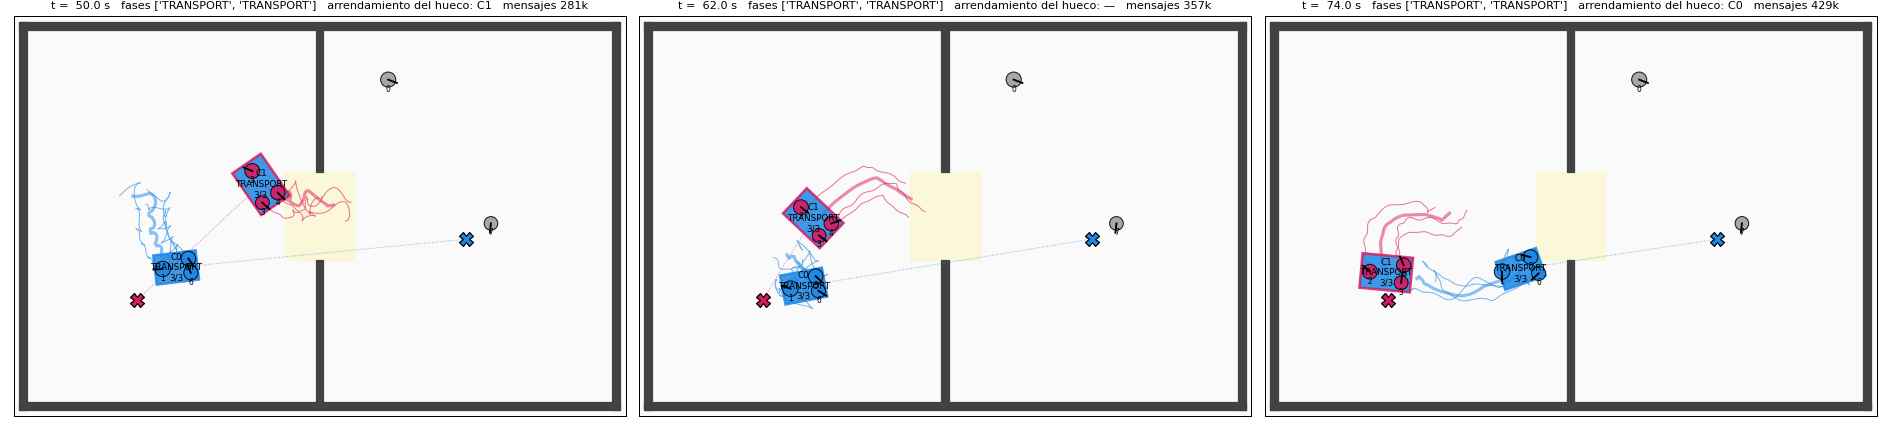
\includegraphics[width=\textwidth]{figs/sim_plan_frames.png}
\caption{La misma semilla 0 con el juego continuo de trayectorias en lugar del
seguidor de puntos (\cref{fig:sim-ref}). Arriba: las rutas de las cargas pasan
de zigzags y bucles frente al vano a curvas largas; C1 cruza primero por el eje
y sale por su carril, C0 espera en el suyo y cruza después. Abajo, tres
instantes ($t=50$, $62$ y $74$~s): la salida de C1, el desvío de C1 alrededor
de C0 —cuyo carril de espera cae sobre el camino al destino de C1— y el
arranque de C0 hacia el vano. Ese desvío es la externalidad atómica actuando:
la continuación publicada de C0 (estática mientras espera) deforma la de C1.}
\label{fig:sim-plan}
\end{figure}
